%%%%%%%% ICML 2022 EXAMPLE LATEX SUBMISSION FILE %%%%%%%%%%%%%%%%%

\documentclass[nohyperref]{article}

% Recommended, but optional, packages for figures and better typesetting:
\usepackage{microtype}
\usepackage{graphicx}
\usepackage{subfigure}
\usepackage{booktabs} % for professional tables

% hyperref makes hyperlinks in the resulting PDF.
% If your build breaks (sometimes temporarily if a hyperlink spans a page)
% please comment out the following usepackage line and replace
% \usepackage{icml2022} with \usepackage[nohyperref]{icml2022} above.
\usepackage{hyperref}


% Attempt to make hyperref and algorithmic work together better:
\newcommand{\theHalgorithm}{\arabic{algorithm}}

% Use the following line for the initial blind version submitted for review:
\usepackage{icml2022}

% If accepted, instead use the following line for the camera-ready submission:
% \usepackage[accepted]{icml2022}

% For theorems and such
\usepackage{amsmath}
\usepackage{amssymb}
\usepackage{mathtools}
\usepackage{amsthm}

% if you use cleveref..
\usepackage[capitalize,noabbrev]{cleveref}

%%%%%%%%%%%%%%%%%%%%%%%%%%%%%%%%
% THEOREMS
%%%%%%%%%%%%%%%%%%%%%%%%%%%%%%%%
\theoremstyle{plain}
\newtheorem{theorem}{Theorem}[section]
\newtheorem{proposition}[theorem]{Proposition}
\newtheorem{lemma}[theorem]{Lemma}
\newtheorem{corollary}[theorem]{Corollary}
\theoremstyle{definition}
\newtheorem{definition}[theorem]{Definition}
%\newtheorem{assumption}[theorem]{Assumption}
\theoremstyle{remark}
\newtheorem{remark}[theorem]{Remark}

% Todonotes is useful during development; simply uncomment the next line
%    and comment out the line below the next line to turn off comments
%\usepackage[disable,textsize=tiny]{todonotes}
\usepackage[textsize=tiny]{todonotes}


% User added packages

\usepackage{relsize}
\usepackage{mathrsfs}

\newcommand{\bm}{ \boldsymbol } 

\newcommand{\Amat}{{\bf A}}
\newcommand{\Bmat}{{\bf B}}
\newcommand{\Cmat}{{\bf C}}
\newcommand{\Dmat}{{\bf D}}
\newcommand{\Emat}{{\bf E}}
\newcommand{\Fmat}{{\bf F}}
\newcommand{\Gmat}{{\bf G}}
\newcommand{\Hmat}{{\bf H}}
\newcommand{\Imat}{{\bf I}}
\newcommand{\Jmat}{{\bf J}}
\newcommand{\Kmat}{{\bf K}}
\newcommand{\Lmat}{{\bf L}}
\newcommand{\Mmat}{{\bf M}}
\newcommand{\Nmat}{{\bf N}}
\newcommand{\Omat}{{\bf O}}
\newcommand{\Pmat}{{\bf P}}
\newcommand{\Qmat}{{\bf Q}}
\newcommand{\Rmat}{{\bf R}}
\newcommand{\Smat}{{\bf S}}
\newcommand{\Tmat}{{\bf T}}
\newcommand{\Umat}{{\bf U}}
\newcommand{\Vmat}{{\bf V}}
\newcommand{\Wmat}{{\bf W}}
\newcommand{\Xmat}{{\bf X}}
\newcommand{\Ymat}{{\bf Y}}
\newcommand{\Zmat}{{\bf Z}}

\newcommand{\av}{{\boldsymbol a}}
\newcommand{\Av}{{\boldsymbol A}}
\newcommand{\Cv}{{\boldsymbol C}}
\newcommand{\bv}{{\boldsymbol b}}
\newcommand{\cv}{{\boldsymbol c}}
\newcommand{\dv}{{\boldsymbol d}}
\newcommand{\ev}{{\boldsymbol e}}
\newcommand{\fv}{{\boldsymbol f}}
\newcommand{\Fv}{{\boldsymbol F}}
\newcommand{\gv}{{\boldsymbol g}}
\newcommand{\hv}{{\boldsymbol h}}
\newcommand{\iv}{{\boldsymbol i}}
\newcommand{\jv}{{\boldsymbol j}}
\newcommand{\kv}{{\boldsymbol k}}
\newcommand{\lv}{{\boldsymbol l}}
\newcommand{\mv}{{\boldsymbol m}}
\newcommand{\nv}{{\boldsymbol n}}
\newcommand{\ov}{{\boldsymbol o}}
\newcommand{\pv}{{\boldsymbol p}}
\newcommand{\qv}{{\boldsymbol q}}
\newcommand{\rv}{{\boldsymbol r}}
\newcommand{\sv}{{\boldsymbol s}}
\newcommand{\tv}{{\boldsymbol t}}
\newcommand{\uv}{{\boldsymbol u}}
\newcommand{\vv}{{\boldsymbol v}}
\newcommand{\wv}{{\boldsymbol w}}
\newcommand{\Wv}{{\boldsymbol W}}
\newcommand{\xv}{{\boldsymbol x}}
\newcommand{\yv}{{\boldsymbol y}}
\newcommand{\Xv}{{\boldsymbol X}}
\newcommand{\Yv}{{\boldsymbol Y}}
\newcommand{\zv}{{\boldsymbol z}}


\newcommand{\Gammamat}{{\boldsymbol \Gamma}}
\newcommand{\Deltamat}{{\boldsymbol \Delta}}
\newcommand{\Thetamat}{{\boldsymbol \Theta}}
\newcommand{\Ximat}{{\boldsymbol \Xi}}
\newcommand{\Pimat}{{\boldsymbol \Pi}}
\newcommand{\Sigmamat}{{\boldsymbol \Sigma}}
\newcommand{\Upsilonmat}{{\boldsymbol \Upsilon}}
\newcommand{\Phimat}{{\boldsymbol \Phi}}
\newcommand{\Psimat}{{\boldsymbol \Psi}}
\newcommand{\Omegamat}{{\boldsymbol \Omega}}
\newcommand{\Lambdamat}{{\boldsymbol \Lambda}}
\newcommand{\zerov}{{\boldsymbol 0}}

\newcommand{\alphav}{{\boldsymbol \alpha}}
\newcommand{\betav}{{\boldsymbol \beta}}
\newcommand{\gammav}{{\boldsymbol \gamma}}
\newcommand{\deltav}{{\boldsymbol \delta}}
\newcommand{\epsilonv}{{\boldsymbol \epsilon}}
\newcommand{\zetav}{{\boldsymbol \zeta}}
\newcommand{\etav}{{\boldsymbol \eta}}
\newcommand{\thetav}{{\boldsymbol \theta}}
\newcommand{\iotav}{{\boldsymbol \iota}}
\newcommand{\kappav}{{\boldsymbol \kappa}}
\newcommand{\lambdav}{{\boldsymbol \lambda}}
\newcommand{\muv}{{\boldsymbol \mu}}
\newcommand{\nuv}{{\boldsymbol \nu}}
\newcommand{\xiv}{{\boldsymbol \xi}}
\newcommand{\omicronv}{{\boldsymbol \omicron}}
\newcommand{\piv}{{\boldsymbol \pi}}
\newcommand{\rhov}{{\boldsymbol \rho}}
\newcommand{\sigmav}{{\boldsymbol \sigma}}
\newcommand{\tauv}{{\boldsymbol \tau}}
\newcommand{\upsilonv}{{\boldsymbol \upsilon}}
\newcommand{\phiv}{{\boldsymbol \phi}}
\newcommand{\chiv}{{\boldsymbol \chi}}
\newcommand{\psiv}{{\boldsymbol \psi}}
\newcommand{\omegav}{{\boldsymbol \omega}}

% Added by Tao
\usepackage{soul}

\newcommand{\Span}{\text{Span}}
\newcommand{\CH}{\mathcal{H}}
\newcommand{\CC}{\mathcal{C}}
\newcommand{\corr}{\text{corr}}
\newcommand{\cov}{\text{cov}}
\newcommand{\EE}{\mathbb{E}}
\newcommand{\rank}{\text{rank}}
\newcommand{\discr}{\text{Discr}}
\newcommand{\gener}{\text{Gener}}
\newcommand{\var}{\text{Var}}
\newcommand{\upmodels}{\perp\!\!\!\perp}
\newcommand{\bs}[1]{\boldsymbol{#1}}
\newcommand{\BR}{\mathbb{R}}
\newcommand{\PP}{\mathbb{P}}
\newcommand{\QQ}{\mathbb{Q}}
\newcommand{\hs}{\text{HS}}
\newcommand{\ud}{\,\text{d}}
\newcommand{\CX}{\mathcal{X}}
\newcommand{\CY}{\mathcal{Y}}
\newcommand{\CZ}{\mathcal{Z}}
\newcommand{\MI}{\text{MI}}
\newcommand{\CE}{\mathcal{E}}
\newcommand{\CF}{\mathcal{F}}
\newcommand{\CS}{\mathcal{S}}
\newcommand{\CP}{\mathcal{P}}
\newcommand{\BZ}{\mathbb{Z}}
%\newcommand{\hs}{\text{HS}}
\newcommand{\supp}{\text{supp}}
\newcommand{\Id}{\text{Id}}
\newcommand{\sign}{\text{sign}}
\newcommand{\KL}{\text{KL}}
\newcommand{\bX}{\mathbb{X}}
\newcommand{\bZ}{\mathbb{Z}}

\newcommand{\Enc}{\text{Enc}}
\newcommand{\Dec}{\text{Dec}}

\newcommand{\GAN}{\text{GAN}}
\newcommand{\AEC}{\text{AE}}
\newcommand{\LIK}{\text{LIK}}
\newcommand{\JSD}{\text{JSD}}
\newcommand{\DFM}{\text{DFM}}

\newcommand{\BS}{\mathbb{S}}
\newcommand{\BH}{\mathbb{H}}
\newcommand{\BB}{\mathbb{B}}

\newcommand{\CB}{\mathcal{B}}

\newcommand{\CM}{\mathcal{M}}


\DeclareMathOperator{\sech}{sech}
\DeclareMathOperator{\csch}{csch}
\DeclareMathOperator{\arcsec}{arcsec}
\DeclareMathOperator{\arccot}{arccot}
\DeclareMathOperator{\arccsc}{arccsc}
\DeclareMathOperator{\arccosh}{arccosh}
\DeclareMathOperator{\arcsinh}{arcsinh}
\DeclareMathOperator{\arctanh}{arctanh}
\DeclareMathOperator{\arcsech}{arcsech}
\DeclareMathOperator{\arccsch}{arccsch}
\DeclareMathOperator{\arccoth}{arccoth} 

\DeclareMathOperator{\logit}{logit} 

\DeclareMathOperator{\argmin}{\arg\min}
\DeclareMathOperator{\argmax}{\arg\max}

%\newcommand{\ELBO}{\text{ELBO}}
%\newcommand{\MLE}{\text{MLE}}
%\newcommand{\NCE}{\text{NCE}}

\newcommand{\CL}{\mathcal{L}}
\newcommand{\CU}{\mathcal{U}}
\newcommand{\CI}{\mathcal{I}}
\newcommand{\CD}{\mathcal{D}}

\newcommand{\BF}{\mathbb{F}}
\newcommand{\CN}{\mathcal{N}}
\newcommand{\CQ}{\mathcal{Q}}


\newcommand{\tr}{\text{tr}}

% for image graphics
\usepackage{tikz}
%\usetikzlibrary{bayesnet}
%\usetikzlibrary{calc}

\theoremstyle{plain}
\newtheorem{thm}{Theorem}[section] % reset theorem numbering for each chapter
\theoremstyle{definition}
\newtheorem{defn}[thm]{Definition} % definition numbers are dependent on theorem numbers
\newtheorem{exmp}[thm]{Example} % same for example numbers
\newtheorem{prop}[thm]{Proposition} % same for example numbers
\newtheorem{assumption}[thm]{Assumption}
\newtheorem{lem}[thm]{Lemma}
\newtheorem{rmk}[thm]{Remark}
\newtheorem{col}[thm]{Corollary}
\newtheorem{prob}[thm]{Problem}


\newcommand{\beq}{\begin{equation}}
\newcommand{\eeq}{\end{equation}}
\newcommand{\beqs}{\begin{eqnarray}}
\newcommand{\eeqs}{\end{eqnarray}}
\newcommand{\barr}{\begin{array}}
\newcommand{\earr}{\end{array}}
% \usepackage[colorlinks]{hyperref}
%\usepackage[colorinlistoftodos]{todonotes}




% Comments
\newcommand{\cytao}[1]{\todo[size=\small, color=green!40]{{\bf Tao:} #1}}


% User defined commands

\newcommand{\infonce}{\texttt{InfoNCE}}

\newcommand{\Iv}{\bs{I}}
\newcommand{\COmega}{\mathcal{\Omega}}
\newcommand{\CTheta}{{\Theta}}

\newcommand{\BD}{\mathbb{D}}
\newcommand{\BX}{\mathbb{X}}
\newcommand{\BTheta}{\mathbb{\Theta}}
\newcommand{\BY}{\mathbb{Y}}
\newcommand{\BQ}{\mathbb{Q}}

\newcommand{\BA}{\texttt{BA}}
\newcommand{\UBA}{\texttt{UBA}}
\newcommand{\TUBA}{\texttt{TUBA}}
\newcommand{\NWJ}{\texttt{NWJ}}
\newcommand{\DV}{\texttt{DV}}
\newcommand{\MINE}{\texttt{MINE}}
\newcommand{\ANCE}{\texttt{$\alpha$-InfoNCE}}
\newcommand{\FLO}{\texttt{FLO}}
\newcommand{\PMI}{\text{PMI}}
%\newcommand{\JSD}{\texttt{JSD}}
\newcommand{\FLAT}{\texttt{FlatNCE}}
\newcommand{\NFL}{\texttt{NFL}}
\newcommand{\DDV}{\texttt{DDV}}
\newcommand{\FDV}{\texttt{FDV}}

\newcommand{\DP}{\text{DP}}

\newcommand{\MNIST}{\texttt{MNIST}}

\newcommand{\SimCLR}{\texttt{SimCLR}}
\newcommand{\MoCo}{\texttt{MoCo}}

\newcommand{\CT}{\mathcal{T}}
\newcommand{\CLN}{\mathcal{LN}}

\newcommand{\post}{\text{post}}
\newcommand{\diag}{\text{diag}}

\newcommand{\SIR}{\text{SIR}}
\newcommand{\SEIR}{\text{SEIR}}

\newcommand{\Prompt}{\texttt{Prompt}}
\newcommand{\Transformer}{\texttt{Transformer}}

\newcommand{\Gv}{\bs{G}}
%\newcommand{\Wv}{W}

\newcommand{\CW}{\mathcal{W}}
\newcommand{\CA}{\mathcal{A}}

\newcommand{\te}{{}^{\text{test}}}
\newcommand{\meta}{\text{meta}}
\newcommand{\base}{\text{base}}
\newcommand{\adapt}{\text{adapt}}
\newcommand{\upper}{\text{upper}}
\newcommand{\metaflo}{\texttt{Meta-FLO} }

\newcommand{\GPT}{\texttt{GPT}}

\newcommand{\tnew}{\text{new}}
\newcommand{\told}{\text{old}}

\newcommand{\train}{\text{train}}



% The \icmltitle you define below is probably too long as a header.
% Therefore, a short form for the running title is supplied here:
%\icmltitlerunning{Meta-FLO: Simple Fast Few-Shot Learning With Stochastic Prompt Network}
\icmltitlerunning{Meta-FLO: Principled Simple Fast Few-Shot Learning With Stochastic Prompt Encoding Networks}

\begin{document}

\twocolumn[
%\icmltitle{Meta-FLO: Simple Few-Shot Learning With Stochastic Prompt Network}
\icmltitle{Meta-FLO: Principled Simple Fast Few-Shot Learning \\With Stochastic Prompt Encoding Networks}

% It is OKAY to include author information, even for blind
% submissions: the style file will automatically remove it for you
% unless you've provided the [accepted] option to the icml2022
% package.

% List of affiliations: The first argument should be a (short)
% identifier you will use later to specify author affiliations
% Academic affiliations should list Department, University, City, Region, Country
% Industry affiliations should list Company, City, Region, Country

% You can specify symbols, otherwise they are numbered in order.
% Ideally, you should not use this facility. Affiliations will be numbered
% in order of appearance and this is the preferred way.
\icmlsetsymbol{equal}{*}

\begin{icmlauthorlist}
\icmlauthor{Firstname1 Lastname1}{equal,yyy}
\icmlauthor{Firstname2 Lastname2}{equal,yyy,comp}
\icmlauthor{Firstname3 Lastname3}{comp}
\icmlauthor{Firstname4 Lastname4}{sch}
\icmlauthor{Firstname5 Lastname5}{yyy}
\icmlauthor{Firstname6 Lastname6}{sch,yyy,comp}
\icmlauthor{Firstname7 Lastname7}{comp}
\icmlauthor{Firstname8 Lastname8}{sch}
\icmlauthor{Firstname8 Lastname8}{yyy,comp}
\end{icmlauthorlist}

\icmlaffiliation{yyy}{Department of XXX, University of YYY, Location, Country}
\icmlaffiliation{comp}{Company Name, Location, Country}
\icmlaffiliation{sch}{School of ZZZ, Institute of WWW, Location, Country}

\icmlcorrespondingauthor{Firstname1 Lastname1}{first1.last1@xxx.edu}
\icmlcorrespondingauthor{Firstname2 Lastname2}{first2.last2@www.uk}

% You may provide any keywords that you
% find helpful for describing your paper; these are used to populate
% the "keywords" metadata in the PDF but will not be shown in the document
\icmlkeywords{Machine Learning, ICML}

\vskip 0.3in
]

% this must go after the closing bracket ] following \twocolumn[ ...

% This command actually creates the footnote in the first column
% listing the affiliations and the copyright notice.
% The command takes one argument, which is text to display at the start of the footnote.
% The \icmlEqualContribution command is standard text for equal contribution.
% Remove it (just {}) if you do not need this facility.

%\printAffiliationsAndNotice{}  % leave blank if no need to mention equal contribution
\printAffiliationsAndNotice{\icmlEqualContribution} % otherwise use the standard text.

%We derive a novel information-theoretic analysis of the generalization property of meta-learning algorithms. Concretely, our analysis proposes a generic under- standing of both the conventional learning-to-learn framework [1] and the modern model-agnostic meta learning (MAML) algorithms [2]. Moreover, we provide a data-dependent generalization bound for a stochastic variant of MAML, which is non-vacuous for deep few-shot learning. As compared to previous bounds that depend on the square norm of gradients, empirical validations on both simulated data and a well-known few-shot benchmark show that the proposed bound is orders of magnitude tighter in most situations.

\begin{abstract}
This work presents a novel meta-learning framework towards quick, robust, principled few-shot generalization via task-level variational contrastive learning. Our proposal, named {\it Meta-FLO}, is distinct from popular meta/few-shot learning approaches in significant ways: it does not rely on any explicit gradient manipulation,  feature space engineering, or external memories. Instead, $\metaflo$ can be simply activated as a plug-in regularizer. Rooted in the information-theoretic learning theory, $\metaflo$ directly targets the generalization performance of meta-learners using the contrastive Fenchel-Legendre Optimization. Our $\metaflo$ does not rely on strong assumptions as in classical regularization frameworks and it is relatively sharp for being data-dependent. To further simplify the design and allow more modeling flexibilities, $\metaflo$ introduces a new architecture called {\it Stochastic Prompt Network} for efficient task encoding. The efficiency and effectiveness of $\metaflo$ are vetted through an extensive set of empirical evaluations, with encouraging results reported. 

%it does not reply on any explicit gradient manipulation as in Model-Agnostic Meta-Learning (MAML),  feature space engineering as in Prototypical Networks, external memories as in Meta Networks. 
%This work introduces a novel variational meta-learning strategy by exploiting task-level and distribution-level contrastive signals. Distinct from prior-arts, our proposal, named {\it Meta-FLO}, explicitly seeks out discrepancies rather than commonalities. To enable this, we bring together ideas from {\it model-agnostic meta-learning} (MAML) and variational mutual information estimation. Seemingly unrelated, we show how these two research topics are connected through ($i$) a data-dependent information-theoretic bound on the generalization risk for meta-learners and ($ii$) tight variational mutual information bound with contrastive estimation. $\metaflo$  generalizes the popular instance-level contrastive training to a more abstract level: it now regards tasks and datasets in the meta-learning scenario as individual data points to extract learning signals. The efficiency and effectiveness of $\metaflo$ is vetted through an extensive set of empirical evaluations, with encouraging results reported. 
\end{abstract}




\section{Introduction}

Quick, robust generalization across different tasks with little supervision is considered as the hallmark signature of human intelligence, and enabling such human-like few-shot learning capability constructs one of the central challenges in modern machine learning. A significant body of research work has been dedicated to attacking this problem, with different focuses on solving the three core issues: ($i$) prime prior knowledge from previously seen tasks; ($ii$) extract useful information from the limited exemplars for a new task; ($iii$) avoid over-fitting the data with powerful learners such as deep nets. Drawing on the recent advances in variational contrastive learning and results of information-theoretic generalization theory, this research investigates a novel scalable few-shot learning framework that is flexible enough for generic machine learning applications. 

%classical generalization bounds based on various notions of complexity of hypothesis set fail to explain this phenomenon. 

To facilitate our discussion, we collectively refer to all techniques that draw prior knowledge from previously seen tasks to facilitate the learning of a new task in sample-scarce scenarios as {\it meta-learning}, which broadly overlaps research topics such as learning to learn \citep{thrun1998learning}, domain adaptation \citep{daume2009frustratingly}, transfer learning \citep{pan2009survey}, causal machine learning \citep{scholkopf2021toward}, zero/few-shot learning \citep{}, weakly supervised learning \citep{robinson2020strength}, {\it etc.} Despite the different modeling assumptions made, a shared theme among these approaches is to extract invariant relations and/or representations that are useful for new, unseen tasks. This heuristic is typically implemented by a two-stage learning procedure: first in the {\it meta-learn phase} the learner $\CF$ captures the invariance under the modeling assumptions made using diverse training tasks $\CD_{\train}$; then in the {\it adaption phase} the meta-learner leverages an adaptation algorithm $\CA$ to compose the learned invariance with the variable part informed by the new task data $\BS$ to derive a solution $F = \CA(\BS;\CF)$. 

Let us contextualize in zero/few-shot learning scenarios\footnote{As an important remark, our discussions can be easily extended to more general meta-learn settings. }, which has garnered considerable attention from both academia and industry in recent years \citep{}. In this setting, $\BS$ can be a few ground-truth examples ({\it i.e.}, few-shot), or a descriptive cue for what are the expected behaviors to accomplish the new task ({\it i.e.}, zero-shot). Simple heuristics on representation invariance/similarity mostly rule in this realm, and they worked pretty well: {\it Neural Turing Machines} \citep{graves2014neural}  and {\it Meta Net} \citep{munkhdalai2017meta} exploited external memories to cache and access meta-info; {\it Matching Net} \citep{munkhdalai2017meta} used attention-based weights on support set to cast votes, while {\it Prototypical Net} \citep{snell2017prototypical} finds the class-centroids in the meta-learned representation space for nearest neighbor classification.  More sophisticated solutions seek to capture relational invariance, for instance {\it Causal Mechanism Transfer} \citep{teshima2020few, xiu2021supercharging} reverse-engineered the invariant causal data generation procedure for statistically consistent data-augmentations to train new tasks. Of particular interest is the works of {\it Model-Agnostic Meta-Learning} (MAML) \citep{finn2017model, nichol2018first, rajeswaran2019meta, raghu2019rapid}, where the goal of meta-train is to find a good parameter initialization for subsequent task adaptations using gradient descent adaptations. 

Despite encouraging progress made, these prior-arts are not without caveats. Sophisticated architectures or algorithms are often entailed \citep{graves2014neural, munkhdalai2017meta, teshima2020few}, thus requiring not only extensive engineering efforts to customize solutions but also implying delicate model tuning. Models relying on augmented memories are bulky and less effective in capturing task invariance \citep{arjovsky2019invariant}. While being more flexible, gradient-based approaches such as MAML typically demand explicit gradients manipulations \citep{zhou2021meta}, and they converge slowly. Importantly, most popular solutions lack principled mechanisms to guard against over-fitting issues, and they almost exclusively rely on the train-validation split paradigm \citep{bai2021important}, which further exacerbates the data-scarcity issue. 



Seeking to improve on current practices, we dive deep to the theoretical roots of meta-learning. Classical generalization theory based on the different complexity measures of model spaces, such as VC dimensions and Rademacher complexity \citep{vapnik1999nature}, generally fails to explain the exceptional generalization ability of modern deep neural networks and meta-learning algorithms \citep{zhang2017understanding}, where the number of parameters can far exceed the number of data samples. Concretely, the observed generalization risk is typically magnitudes better than theoretical predictions made by the VC bounds \citep{}. To bridge this gap, information-theoretic generalization theory emerged as a powerful mathematical tool for theoretical analysis. While strong empirical evidence indicates such theories adequately capture the observed generalization behaviors of deep learners and popular meta-learning frameworks, a critical limitation of these studies is that they typically only shed theoretical insights rather than offering practical gains, as the presented theories often do not materialize into efficient algorithms that directly helps the training of meta-learners. This difficulty arises because information-theoretic bounds often crucially relies on information quantities that are challenging to compute let alone optimize in high-dimensions, such as the Shannon mutual information. 

%xu2017information, harutyunyan2021information

%lee2019meta


%This difficulty arises because ITGT bounds crucially relies on the mutual information between the 


Our work is inspired by the recent successes of two seemly unrelated streams of research: {\it contrastive learning} \citep{oord2018representation, chen2020simple} and {\it prompt-tuning} \citep{sanh2021multitask}. Contrastive learning exploits the idea of comparing positive and negative samples to capture subtle features for representation optimization, which is theoretically justified as optimizing the mutual information for the input pairs \citep{poole2019variational, guo2021tight}. On the other hand, prompt-tuning made the exciting empirical discovery that large-scale pre-trained language models are excellent few-shot learners \citep{liu2021pre}: by prompting the language models with gold examples or cues for the expected outputs, they can quickly learn to adapt to unseen tasks. We bring these ideas together to build a novel contrastive meta-learning framework that not only overcomes the respective limitations described above but also formalizes and extends the emerging few-shot capabilities of prompt-tuning to benefit generic learning tasks. Our contributions highlight:
\begin{itemize}
\setlength\itemsep{0pt}
\item A principled plug-in regularizer for easy meta-learning
\item A prompt encoding network for one-step adaptation
\item A careful analysis of generalization to guide practices
\end{itemize}
Our work non-trivially integrates recent theoretical and empirical results to derive a simple yet strong-performing meta-learning solution: to the best of our knowledge, this is the first work that moves beyond instance-level contrastive learning and the only trainable information-theoretic generalization objective for meta-learning. To further assist in unlocking potentials, we release codes that are immediately compatible with most machine learning applications, enabling a frictionless, robust meta-learning experience with minimal code changes compared to competing solutions. 



\begin{figure*}[t!]
%\includegraphics[trim=0 .5in 7in 3in, clip, height=1.5in]{figures/cartoon/latent_causal_models}
\begin{center}
{
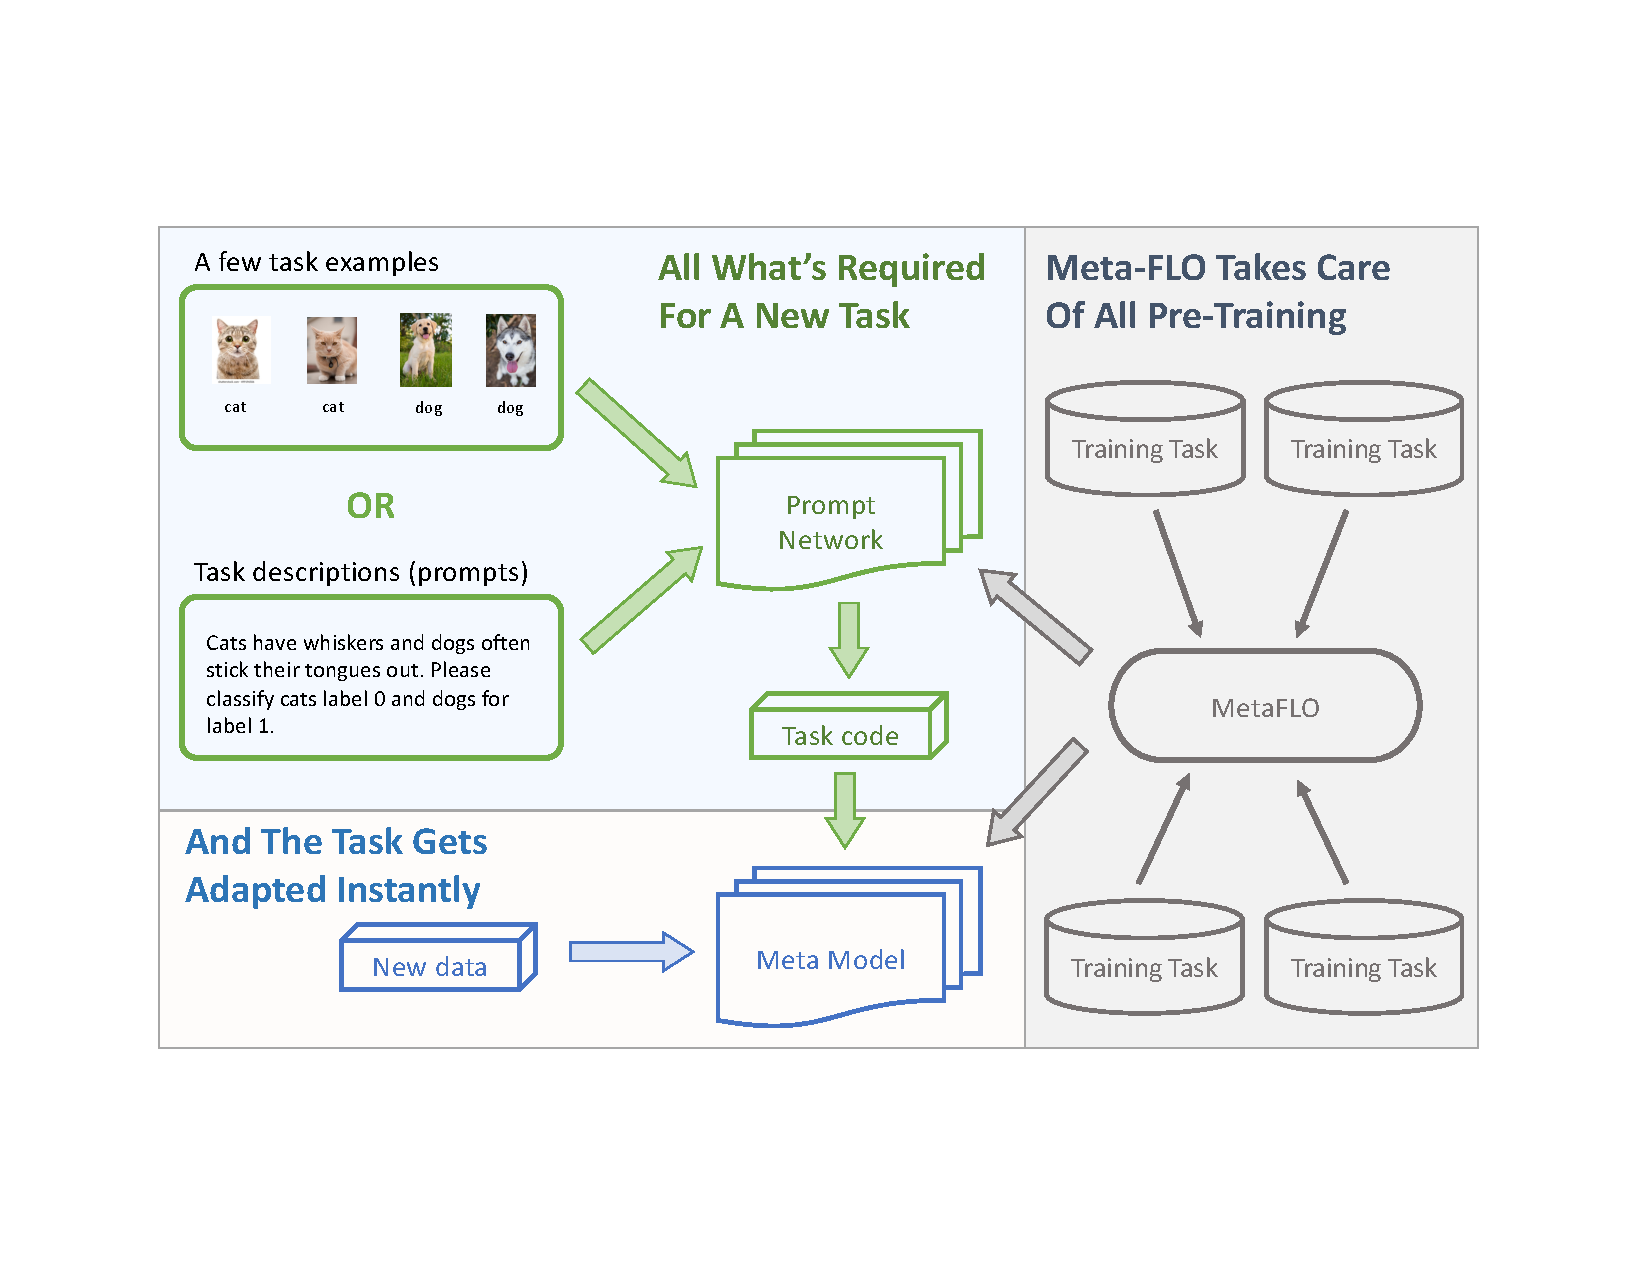
\includegraphics[width=.9\textwidth]{figures/metaflo-demo}
}
\end{center}
%\vskip -.1in
%\caption{.}
\vspace{-1.5em}
\caption{Schematic plot of $\metaflo$ framework. \label{fig:metaflo}}
\vspace{-1.em}
\end{figure*}


%\section{Information-Theoretic Generalization Theory For Meta-Learning}
\section{Preliminaries}

This section briefly reviews required technical backgrounds. 
%We use capital letters to denote random variables. 

%{\bf Generalization bounds for meta-learning.} 
\subsection{Information-theoretic generalization theory \\\hspace{1.8em}for meta-learning}

Consider task distribution $\mu_t(z)$ defined on an instance space $\CZ = \CX \times \CY$, where $t$ is the task identifier and $z=(x, y)$ is the (feature, label) pair. Following standard notations, we use capital letters for random variables ($X, Y, Z, \cdots$) and lower case letters for realizations ($x, y, z, \cdots$).  Let $\BS_t = \{ Z_i \}_{i=1}^m \sim \mu_t^m$ be a set of $m$ independent samples drawn from $\mu_t$, which we identify as the training dataset, which is also known as the {\it support set}, or an {\it episode}, in meta/few-shot learning contexts\footnote{With slight abuse of notation, we also use $\BS$ to denote a realization of training data ({\it i.e.}, $\{ z_i \}_{i=1}^m$), which simplifies the text.}. 
%and a set of independent samples $\BS = \{ Z_i \}_{i=1}^m$ drawn from $\mu_t$. 
Given a model space $\CM$ and a loss function $\ell: \CM \times \CZ \rightarrow \BR$, the true risk and the empirical risk of $f\in \CM$ are respectively defined as $R_{t}(f) \triangleq \EE_{Z\sim\mu_t}[\ell(f, Z)]$ and $\hat{R}_t(f;\BS_t) \triangleq \frac{1}{m} \sum_{i=1}^m \ell(f, Z_i)$. For now let us set focus on the general as oppose to task-specific learning by dropping the subscript $t$. An algorithm $\CA$ is a randomized mapping that takes a dataset $\BS$ as input and outputs a model $f\in \CM$ accordingly to a conditional distribution $p_{\CA}(f|\BS)$, that is $F=\CA(\BS)\sim p_{\CA}(f|\BS)$. For instance, {\it standard stochastic gradient descent} (SGD) defines such a random algorithm. A subset of $\BS_t$, or additional independent draws from the same task distribution, will be used for the loss evaluation. We identify this dataset as the {\it query set} or {\it validation data}, denoted by $\BQ_t$. The expected generalization error for task $t$ with learning algorithm $\CA$ is then defined as $G(\mu_t, \CA)\triangleq \EE_{F_t,\BS_t}[R_t(F_t)-\hat{R}_t(F_t;\BS_t)]$. The seminal work of \citet{xu2017information} first characterized the connection between the generalization risk and the information-theoretic metrics, as summarized below\footnote{We defer some of the technical definitions to the Appendix.}:
%$\mathscr{S}$
%$\mathcal{S}$

\begin{thm}[\citet{xu2017information}]
Suppose that for each $f\in \CM$, the prediction loss $\ell(f,Z)$ is $\sigma$-subgaussian with respect to $Z\sim \mu$. Then for any randomized learner $\CA$ characterized by $p_{\CA}(f|\BS)$, for $\BS\sim\mu^m$, we have 
\beq
|G(\mu, \CA)| \leq \sqrt{\frac{2\sigma^2}{m} I(F;\BS)}, 
\eeq
where $I(F;\BS)$ is the Shannon mutual information ({\it c.f.}, Eq. (\ref{eq:mi})) between the input and output of algorithm $\CA$. 
\end{thm}
This result basically says that the less output $F$ depends on dataset $\BS$, the smaller the generalization error of $\CA$ will be. This is intuitive: consider an algorithm that outputs a constant $f$ regardless of the input, then $R=\hat{R}$ so there is no generalization error. However, for an algorithm $\CA$ to be useful, model $F$ must learn from train data $\BS$, and consequently $I(F;\BS)>0$. With a more powerful learner, $\hat{R}$ will be smaller but $I(F;\BS)$ will be larger, so in the low-sample regime ({\it i.e.}, small $m$) the model is expected to generalize poorly, which is more commonly known as over-fitting the data. Note such information-theoretic generalization theories have been mostly used for theoretical analyses rather than deriving useful algorithms, because ($i$) computing $I(F;\BS)$ is considered practically challenging; and ($ii$) in practice we only have one training dataset, which renders the (one-shot) estimation of mutual information an ill-posed problem. These are the key challenges we seek to address in the current paper.


Now let us get contextualized in the meta-learning setting. Let $\tau$ be the distribution where all tasks originate (known as the {\it environment} in some contexts), {\it i.e.}, $t \sim \tau(t)$. For meta-learning, we sample $n$-tasks for training and $n'$-tasks for testing, respectively denoted as $\BS_{1:n}$ and $\BS\te_{1:n'}$. We further decouple the learning algorithm into two parts: the {\it meta-learner} $\CA_{\meta}(\BS_{1:n})$ that consumes all train data to get the {\it meta-model} $f_{\meta}$, and then {\it task-adaptation learner} $\CA_{\adapt}(f_{\meta}, \BS_t)$ which adapts the meta-model to the individual task data $\BS_t$ to get task model $f_t$. For parameterized models such as deep nets, we denote $\Theta$ as our {\it meta parameters} and $E_t$ as {\it task-parameters}, that is to say $\Theta \triangleq \CA_{\meta}(\BS_{1:n})$, $E_t \triangleq \CA_{\base}(\Theta, \BS_t)$, where $\Theta, E_t$ can be understood as weights of deep nets. In subsequent discussions, we will also call $E_t$ the {\it task-embedding}. We can define the population {\it meta-risk} as $R_{\tau}(\Theta) \triangleq \EE_{t, \Theta=\CA_{\meta}(\BS_{1:n})}[\EE_{E_t=\CA_{\adapt}(\Theta,\BS_t)}[R_{t}(f_{E_t})]]$, and similarly for the empirical risk $\hat{R}_{\tau}$ evaluated on the query set $\BQ_t$. The following result on the expected generalization risk $G(\tau, \CA_{\meta}, \CA_{\adapt}) \triangleq \EE[R_\tau-\hat{R}_{\tau}]$ adapted from \citet{chen2021generalization} lays the theoretical foundation of our work, to be exploited in Sec \ref{sec:metaflo}. 

%$S\sim\mu_{m,\tau}$, $m$ data points in $S$ that are independently sampled from a random task $\mu$ encountered in $\tau$. 


%For meta-learning, we use the {\it meta parameter} $\Theta$ to represent the shared knowledge, and $W_{1:n}$ the task specific knowledge. Let us denote $\Theta \triangleq \CA_{\meta}(S_{1:n})$, $W = \CA_{\base}(\Theta, S)$, and the meta-risk $R_{\tau}(\Theta) \triangleq \EE_{\mu, S}[\EE_{W=\CA_{\base}(\Theta,S)}[R_{\mu}(W)]]$. The following statement provides an upper bound for meta-learning generalization risk. 

\begin{thm}[\citet{chen2021generalization}, Theorem 5.1]
Suppose all tasks use the same loss $\ell(Z,w)$, which is $\sigma$-subgaussian for each $e\in\CE$, where $Z\sim\mu_t, t\sim\tau$. Then, the meta generalization error for joint training is upper bounded by 
\beq
|G(\tau, \CA_{\meta}, \CA_{\base}) | \leq \sqrt{\frac{2\sigma^2}{nm}I(\Theta, E_{1:n};\BS_{1:n})}.
\label{eq:meta_bound}
\eeq
By the chain rule of mutual information, this error bound can be further relaxed to 
\beq
\begin{array}{l}
\sqrt{\frac{2\sigma^2}{mn}(I(\Theta;\BS_{1:n})+\sum_i I(E_{t_i};\BS_{t_i}|\Theta))} \leq \\
[5pt]
\hspace{2em}\sqrt{\frac{2 \sigma^2}{mn}I(\Theta;\BS_{1:n})} + \sqrt{\frac{2\sigma^2}{mn}\sum_i I(E_{t_i};\BS_{t_i}|\Theta)}
\end{array}
\label{eq:meta_bound}
\eeq
\end{thm}


\subsection{Contrastive mutual information estimation} 

Switching gears, let us talk about how to assess the dependency between pairs of variables, which is integral for many scientific and engineering endeavors \citep{reshef2011detecting}. The Shannon {\it mutual information} (MI) 
\beq
I(X;Y) \triangleq \EE_{p(x,y)}\left[\log \frac{p(x,y)}{p(x)p(y)}\right] \label{eq:mi} 
\eeq
has been established as a popular metric to quantify such generic associations \citep{shannon1948mathematical}. To scale MI estimation to the ever-growing size and complexity of modern datasets, variational objectives have gained wide popularity in recent years \citep{oord2018representation}. These approaches appeal to various variational inequalities to construct tractable \& differentiable lower or upper bounds of the mutual information \citep{poole2019variational}, thus turning the estimation of MI into an optimization problem. Of particular interest are the contrastive variational estimators, where pairs of positive samples (drawn from $p(x,y)$) and negatives samples (drawn from $p(x) p(y)$) are explicitly contrasted via a critic function $g(x,y)$ to derive MI bounds. For example, the popular $K$-sample $\infonce$ objective takes the form
\beq
%I_{\infonce}^K(X;Y) = \EE_{p^K(x,y)}\mathlarger{\mathlarger[}\underbrace{-\log \frac{1}{K}\sum\nolimits_{k'} \exp(\overbrace{g(x_1, y_{k'})-g(x_1, y_1)}^{\text{Contrast}})}_{I_K(\{(x_k, y_k)\})}\mathlarger{\mathlarger]} , 
\label{eq:infonce}
\begin{array}{c}
\hat{I}_{\infonce}^K(X;Y|g)\triangleq \frac{1}{K}\sum_i \left[\log \frac{e^{g(x_i,y_i)}}{\frac{1}{K}\sum_{k} e^{g(x_{i}, y_{k})}}\right] \leq I(X;Y), \\
%I_{\infonce}^K(X;Y) \triangleq \max_{f\in \CF} \{I_{\infonce}^K(X;Y|f)\}, 
\end{array}
\eeq
where $(x_i, y_i)$ are paired positive samples and the critic function $g(x,y)$ is optimized to tighten the estimate. Intuitively, the critic $g(x,y)$ predicts whether a sample is positive or negative, similar to its counterpart {\it discriminator} in GAN models \citep{goodfellow2014generative}. Such contrastive estimation strategy is known to be very sensitive in capturing subtle associations, thus making it suited for representation learning applications \citep{gutmann2010noise, mnih2013learning, chen2020simple}. Practically, variational contrastive objectives are easy to implement, enjoy fast algorithms, and importantly they yield much lower variance compared to alternative estimators \citep{guo2021tight}. 

Despite its popularity, the $\infonce$ estimator is known to suffer from the $\log$-$K$ curse \citep{oord2018representation, chen2021simpler}, that is $\hat{I}_{\infonce}^K(X;Y|g) \leq \log K$.
%\beq
%\hat{I}_{\infonce}^K(X;Y|g) \leq \log K.
%\eeq
This implies to reliably estimate MI, the sample size ({\it i.e.}, the batch-size in the training of deep networks) needs to be sufficiently large. While technically possible, this can be very costly: in prominent applications of $\infonce$, achieving reasonable performance entails large batch training and massive parallelization ($\it e.g.$, prominent works like $\SimCLR$ \citep{chen2020simple} and $\MoCo$ \citep{he2020momentum} used mini batch-size ranging between $4k-65k$ for standard vision model pre-training). If we are to use $\infonce$ for the MI term in Eq. (\ref{eq:meta_bound}), it quickly renders the computation unaffordable: this means loading a large number of episodes at a time, each containing multiple data instances for the corresponding task. Such a brute-force application easily blows up memory on computing devices. 

%If we are to use the generalization bounds for meta-learning, this becomes unaffordable, as the MI needs to be estimated at task-level (known as episodes in meta-learning settings): since multiple data instances are involved in each episode, very few episodes can be loaded in each batch before it blows up memory on the computing device. Consequently, it results in poor estimate of the MI term in Eq. (\ref{eq:meta_bound}). 

As such, we appeal to a recent generalization of $\infonce$ known as the $\FLO$ estimator \citep{guo2021tight}. $\FLO$ leverages the Fenchel-Legendre Optimization technique that gives tight, low-variance, unbiased estimation of MI regardless of batch-size $K$ \citep{fenchel1949conjugate, tao2019fenchel}. Theoretically, $\FLO$'s theory encompasses other popular variational MI bounds ({\it e.g.}, $\DV$, $\NWJ$, $\TUBA$, and $\infonce$), and it is the only known trainable MI estimator that provably converges with stochastic gradient descent. We summarize an efficient $\FLO$ implementation in Algorithm \ref{alg:flo} and refer interested readers to Appendix for technical details. 

%effectively turns $K$ into infinite with an arbitrary mini batch-size $B$ \citep{fenchel1949conjugate, tao2019fenchel}. Technically, when adequately optimized, $\FLO$ is an unbiased estimate of MI regardless of batch-size, and it is the only known trainable MI estimator that provably converges under standard technical conditions. We summarize the $\FLO$ in Algorithm \ref{alg:flo} and refer interested readers to Appendix for technical details and more efficient implementations. 

  \begin{algorithm}[t!]
%   \caption{Fenchel-InfoNCE}
\caption{$\FLO$ mutual information estimation}
   \label{alg:flo}
\begin{algorithmic}
%\small
\STATE Empirical data $\hat{p}_d = \{ (x_i, y_i) \}_{i=1}^n$ \\
[1pt]
\STATE Model parameters $\Psi = (\theta, \phi)$ \\
[1pt]
\FOR{$t=1,2,\cdots$}
\STATE Sample $i,i' \sim [n]$ \\
[1pt]
\STATE $u = u_{\phi}(x_i), g_{\oplus} = g_{\theta}(x_i, y_i)$, \\
\STATE $g_{\ominus} = g_{\theta}(x_i, y_{i'})$\\
[1pt]
\STATE $\CF = u + \exp(-u+g_{\ominus}-g_{\oplus})$\\
[1pt]
$\Psi_{t} = \Psi_{t} - \eta_t \nabla_{\Psi} \CF$
\ENDFOR\\
\STATE $\hat{I}_{\FLO} = -\hat{\EE}[\CF]$+1
\end{algorithmic}
\end{algorithm}
%\vspace{-1em}

\section{Meta-FLO}
\label{sec:metaflo}

{\bf Intuitions.} Now we are ready to describe our new solution for meta-learning. Recall from the last section, $R_{\tau}$ is the generalization error and $\hat{R}_{\tau}$ is the empirical estimate.  Our heuristic is simple, that is to optimize a tractable upper bound of the generalization risk given by
\beq
R_{\tau} \leq \underbrace{\hat{R}_{\tau}}_{\text{Utility}} + \underbrace{| R_{\tau}  - \hat{R}_{\tau}  |}_{\text{Generalization}} \triangleq \CL_{\upper}. 
\label{eq:upper}
\eeq
We can consider $\CL_{\upper}$ as a recapitalization of the standard utility-generalization trade-offs in machine learning. To retain necessary rigor, some technical conditions are in order. 

%In meta-learning, we are interested in the population risk $R = \EE_{t\sim\tau}[R_{t}]$, where $t$ is the task identifier and $\tau(t)$ is a distribution of all tasks. which can be estimated with empirical estimate $\hat{R} = \frac{1}{n} \sum_{i} \hat{R}_{t_i}$, where $\hat{R}_i \triangleq \frac{1}{K} \sum_k \ell(\hat{w}_i, z_{i,k})$ is the task-specific risk estimate. An upper bound of $R$ can be readily derived by
%\beq
%%R = R - \hat{R} + \hat{R} \leq \hat{R} + |R - \hat{R}|
%R \leq \hat{R} + |R - \hat{R}| \triangleq \CL_U, 
%\eeq
%which recapitalizes the standard utility-generalization trade-offs in machine learning. For instance, a trivial solution where model parameter $w$ is fixed to a constant will have zero generalization error, but it is not very useful because it can not make task-specific predictions ({\it i.e.}, the empirical risk $\hat{R}$ will be large and consequently diminished utility). 

%({\it i.e.}, $|R - \hat{R}|=0$ )

\begin{assumption}[Task homogeneity\label{thm:assumption}] $I(E_t;\BS_t|\Theta) = I(E_{t'};\BS_{t'}|\Theta) $ for all $t, t' \sim \tau$. 
%\begin{itemize}
%\item {\it Homogeneity. } $I(W_i;S_i|U) = I(W_j;S_j|U)$ 
%%$I(W_i;S_i|U) = I(W_j;)$
%\end{itemize}
\end{assumption}

We make this assumption because the generalization term in Eq. (\ref{eq:upper}) is essentailly the $G(\tau, \CA_{\meta}, \CA_{\base})$ from Eq. (\ref{eq:meta_bound}), which can be bounded from above with 
\beq
%\sqrt{\frac{2 \sigma^2}{mn}I(\Theta;\BS_{1:n})} + \sqrt{\frac{2\sigma^2}{mn}\sum_i I(E_{t_i};\BS_{t_i}|\Theta)}. 
\underbrace{\sqrt{\frac{2 \sigma^2}{mn}I(\Theta;\BS_{1:n})}}_{\text{{\it meta-generalization gap}}} + \underbrace{\sqrt{\frac{2\sigma^2}{mn}\sum_i I(E_{t_i};\BS_{t_i}|\Theta)}}_{\text{{\it task-generalization gap}}}. 
\label{eq:gaps}
\eeq
Thus {\it Assumption } \ref{thm:assumption} allows us to reduce the terms in task-generalization gap above into a single statistics $I(E;\BS|\Theta)$, which can be efficiently estimated and then differentiably optimized using training task samples. 

%To simplify our discussion, let us refer to the the two terms in Eq. (\ref{eq:gaps}) respectively as the {\it meta-generalization gap} and the {\it task-generalization gap}. While we can not possibly estimate or bound the meta-generalization gap, {\it Assumption } \ref{thm:assumption} allows us to simplify the task-generalization gap to a single statistics $I(E;\BS|\Theta)$, which can be efficiently estimated and then differentiably optimized using training task samples. The remainder of this section provides a detailed recipe to construct such an MI-based generalization objective. 


Our reasoning is as follows: in a typical meta-learning scenario one has access to abundant training tasks, but perhaps very few training instances per task (the large $n$ small $m$ case). In this case, fortunately, the intractable base generalization gap $\sqrt{\frac{2 \sigma^2}{mn}I(\Theta;\BS_{1:n})}$ will diminish with an increasing episode size $n$, but the task generalization gap becomes fixed to $\sqrt{\frac{2\sigma^2}{m} I(E;\BS|\Theta)}$  since we only have limited sample size $m$ for each task. Consequently, it is more important to regularize the task generalization gap from Eq. (\ref{eq:gaps}) in typical few-shot learning scenarios, where the training tasks are abundant but individual supervisions may be insufficient for each task. 

{\bf $\metaflo$ loss.} Such motivated, we propose to optimize the following MI-regularized loss, which asymptotically upper bounds the generalization risk by appealing to Eq. (\ref{eq:upper})
\beq
\begin{array}{l}
\CL_{\texttt{Meta-FLO}}(\theta, \CA_{\adapt}) = \\
[5pt]
\hspace{3em}\EE_{\BS}\left[\hat{R}(f_{\theta, \CA_{\adapt}};\BS_{1:n}) + \lambda \sqrt{\hat{I}_{\FLO}(E; \BS)}\right], 
\end{array}
\eeq
where $\theta$ is the meta-model parameters, $\CA_{\adapt}$ is the adaptation mechanism for tasks, and $\lambda>0$ is the regularization strength either computed from $(\sigma^2, m)$ or tuned as a hyper-parameter.  Note that we have suppressed the notation for commensally optimized $\FLO$-parameters $\phi$ for clarity.
While the above optimization target seems conceptually easy, significant challenges are involved with the numerical estimation and optimization of $I(E;\BS)$: the size and structure of $E$ and $\BS$ make them not directly amendable to standard MI-estimation procedures. In typical deep learning scenarios, $E$ is the parameters of a neural network, and $\BS$ is essentially an empirical dataset comprised of a few training samples. These render MI estimation intractable as $E$ resides in an ultra high-dimensional space, and $\BS$ may have variable sizes. The remainder of this section is dedicated to a detailed recipe to construct a highly-efficient MI-based meta-learning objective. 
%Below we detail our design choices to overcome such difficulties.

%commensally






{\bf Overall architecture.} The workflow of our $\metaflo$ model is straightforward: first, $(a)$ we embed task parameters and support data to low dimensional vectors respectively as $e_t=\texttt{Prompt}(\BS_t, \xi)$ (task) and $v_t = \texttt{Prompt}(\BS_t)$ (data) using an architecture called prompt encoder; and ($b$) the task predictions on the query set are made with meta-model $f_{\theta}$ that takes an extra input for task embedding, {\it i.e.}, $\hat{y} = f_{\theta}(x, e_t)$; then ($c$) apply variational contrastive MI estimator $\FLO$ on the $(e_t, v_t)$ to assess MI between the task and support data; and finally, $(d)$ we optimize the MI-regularized empirical loss $\CL_\metaflo$ as a surrogate for the generalization risk upper bound. We summarize the pseudo code in Algorithm \ref{alg:metaflo}. 
%We broke down individual pieces into sections below. 


\begin{algorithm}[t!]
%   \caption{Fenchel-InfoNCE}
\caption{$\metaflo$}
   \label{alg:metaflo}
\begin{algorithmic}
%\small
%\STATE Data $\{ S_i = \{ (x_{i,k}, y_{i,k}) \}_{k=1}^K \}_{i=1}^N$\\
\STATE \# Activating meta-learning in a few lines of code
\STATE Data $\{ S_t = \{ z_{t,k} \}_{k=1}^K \}_{t=1}^N$ where $(X_{t}, Y_{t}) = S_t$\\
%\STATE Meta-parameter $\theta$ %, task-embedding $\{ \phi_t \}_{t=1}^N$\\
\STATE \# Meta-model and Prompt param $\theta$,  $\FLO$ param $\phi$
\STATE \# Prediction model $f_{\theta}(x, e)$, loss function $\ell(\hat{y}, y)$\\
%\STATE Prompt encoder $\Omega_{\phi}$\\
%\STATE \# Pre-compute dataset embedding \\
%\STATE $h_t = \texttt{RKHS\_Embedder}(S_t, \kappa, \text{args})$ \\
[3pt]
%\STATE Initialize parameters $\theta, b$ \\
%\#\#\#\#\# Training \#\#\#\#\#
%\STATE $\BZ = \Enc$
\FOR{$\text{step}=1,2,\cdots$}
%\STATE Sample task mini-batch $\{S_{t_i}\}_{i=1}^B$\\[1pt]
%\STATE \# Sample task data $\underbrace{(X_s^t, Y_s^t)}_{\text{support}}, \underbrace{(X_q^t, Y_q^t)}_{\text{query}}$
%\STATE $\CL_R = \sum_i \ell(f_{\theta}(X_{t_i}, \phi_{t_i}), Y_{t_i})$
\STATE \# Sample support and query data for a task
\STATE \# They are allowed to overlap in $\metaflo$
\STATE \# Support data can be replaced with prompts
\STATE Draw support set $(X_t^s, Y_t^s)$, query set $(X_t^q, Y_t^q)$ %from $p_t$
\STATE \# Prompt encoding, $\xi$ is random noise
\STATE $e_t = \Prompt_{\theta}(X_t^s, Y_t^s, \xi)$ 
\STATE $\CL_R = \sum_i \ell(f_{\theta}(X_t^q, e_t), Y_t^q)$
\STATE $\CL_{\FLO} = \FLO_{\phi}([X_t^s, Y_t^s], e_t)$
%\STATE Sample $(x_{i_t}, y_{i_t}) \sim \hat{p}_{d}(x,y)$, $y_{i_t'} \sim \hat{p}_d(y)$\\
%\STATE Sample $i,i_k' \sim [1, \cdots, n], k\in[1, \cdots, K]$ \\
\STATE $\CL_{\text{Meta-FLO}} = \CL_R + \lambda \sqrt{\CL_{\FLO}}$
\STATE \# Meta-update
\STATE $\text{Optimizer}(\CL_{\text{Meta-FLO}} , \text{params}=[\theta])$
\STATE \# $\FLO$-update
\STATE $\text{Optimizer}(-\CL_{\FLO}, \text{params}=[\phi])$
%\STATE $\gv_{\oplus} = g_{\theta}(x_i, y_i) \in \BR^{m\times 1}$ \\
%\STATE $\gv_{\ominus} = g_{\theta}(x_i, y_{i_k'}) \in \BR^{m \times K}$\\
%\STATE $\gv_{\oplus} = g_{\theta}(x_i, y_i), \gv_{\ominus} = g_{\theta}(x_i, y_{i_k'})$\\
%[1pt]
%\STATE \# $\texttt{logits} = [\gv_{\oplus}, \gv_{\ominus} ], \texttt{labels} = \bs{0}$ \\
%%\STATE 
%\STATE \# $\ell_{\infonce} = \texttt{CrossEntropy}( \texttt{logits}, \texttt{labels})$ \\
%[1pt]
%%\STATE \# $\ell_{\infonce} = \texttt{CrossEntropy}( [\gv_{\oplus}, \gv_{\ominus} ], \bs{0})$ \\
%%\STATE $\texttt{clogits} = \texttt{logsumexp}(\gv_{\ominus} - \gv_{\oplus})$
%\STATE $\texttt{clogits} = \texttt{logsumexp}(\gv_{\ominus} - \gv_{\oplus})$\\
%[1pt]
%%\STATE $\ell_{\FLAT} = \texttt{c}/\texttt{detach}[\texttt{c}], \texttt{c} = \exp(\texttt{clogits})$
%\STATE $\ell_{\FLAT} = \exp(\texttt{clogits}-\texttt{detach}[\texttt{clogits}])$ \\
%[1pt]
%\STATE \# Use your favorite optimizer
%[1pt]
%\STATE $\CF = u + \exp(-u+g_{\ominus}-g_{\oplus})$\\
%[1pt]
%$\Psi_{t} = \Psi_{t} - \eta_t \nabla_{\Psi} \CF$
\ENDFOR
%\STATE {\bf function} $\infonce(\gv_{\oplus}, \gv_{\ominus})$
%\STATE  \hspace{1em} $\texttt{logits} = [\gv_{\oplus}, \gv_{\ominus} ], \texttt{labels} = \bs{0}$
%\STATE \hspace{1em} $\ell_{\infonce} = \texttt{CrossEntropy}( \texttt{logits}, \texttt{labels})$ \\
%\STATE {\bf end function}
%\STATE {\bf function} $\FLAT(\gv_{\oplus}, \gv_{\ominus})$
%\STATE  \hspace{1em} $\texttt{clogits} = \texttt{logsumexp}(\gv_{\ominus} - \gv_{\oplus})$
%\STATE \hspace{1em} $\ell_{\FLAT} = \exp(\texttt{clogits}-\texttt{detach}[\texttt{clogits}])$
%\STATE {\bf end function}
\end{algorithmic}
\end{algorithm}

% ({\it a.k.a}, distribution)

%\subsection{Task/data embedding with Prompt Encoding Nets}


%we fix solutions to a specific architecture $f(x, w)$, where $x$ is the inputs as usual and $w\in \BR^d$ is a task-specific vector we call the task embedding, or prompt vectors. 
%{\bf Task and data embeddings.} 

{\bf Embedding individual tasks and support data.} At a high level, each task is characterized by (an infinite number of) data points from the corresponding task data distribution. This connection allows us to employ similar techniques for both task and dataset embeddings. To motivate the final solution, we first describe a na\"ive task embedding strategy. 

% (formally the $\Theta$ variable in Eq. (\ref{eq:meta_bound})). 

%Note that the task embedding is computed from the 

%To assess the mutual information, 
%There are two ways to get the embedding vector $w_t$ for each task $t$:
%\begin{itemize}
%\item {\it Direct optimization}: make $\{w_t\}$ trainable and update them with 
%\end{itemize}
Note the embedding vector $e_t=\CA_{\adapt}(\BS_t)$ for each task $t$ is derived based on the support set data $\BS_t$ through adaptation mechanism $\CA_{\adapt}$. A popular mechanism widely adopted in meta-learning literature is to make $\{ e_t \}$ trainable and then update them with gradient-based optimizations with respect to empirical task risk $\hat{R}_t(f_{e_t})$. For instance, MAML \citep{finn2017model} treats meta-parameter $\theta$ as initialization and adapt to individual task with $e_t = \theta - \eta \nabla_{\theta} \hat{R}_t(\BS_t)$, where $\eta$ is the hyper-parameter of adaptation rate. While proved useful in many empirical settings, we know this practice is sub-optimal from an information-theoretic generalization perspective: ($i$) computationally, it entails second-order gradients for the meta-parameter updates \citep{nichol2018first}; ($ii$) the deterministic update for $e_t$ implies $I(E;\BS)=\infty$, so there is no protection against overfitting. ($i$) has inspired many low-order gradient approximations to speed up training \citep{rajeswaran2019meta, zhou2021meta}, and MAML exclusively relies on train-validation split to mitigate ($ii$) \citep{bai2021important}. In terms of flexibility, the MAML architecture prohibits zero-shot applications, where one only has the meta-descriptions of the task, but no gold training examples. 


Our considerations for improvements are three-fold: ($a$) to circumvent the difficulty of encoding all parameters of an entire neural network; ($b$) to make our task embeddings uncertainty-aware thus robust against overfitting; ($c$) we want to make adaptation gradient-free for computational efficiency, and flexible enough for zero-shot adaptation. For the first point, we summarize each task $t$ into a fixed-length vector $e_t \in \BR^d$, inspired by the word embedding technique from NLP where tasks are now considered as tokens. This not only makes the estimation of MI tractable but also leverages the embedding space continuity to exploit task similarities. So in addition to the input $x$, we consider a model parameterization that further takes the embedding vector $e$ for the task specification, {\it i.e.}, $f_{\theta}(x, e)$, where $\theta$ is the meta-parameter shared across all tasks from Eq. (\ref{eq:meta_bound}). For the other two points, we propose a novel {\it stochastic prompt encoding network} architecture detailed below to directly infer task embeddings from support data. 

%The most generic approach is to make $\{ e_t \}$ trainable and then update them with SGD or SGLD, which provides the desired randomness to avoid degenerated solutions\footnote{If $w$ is uniquely defined by the support data $S_t$ then MI is $\infty$.}. 
%At inference time, the common practice is to similarly update a (randomly) initialized $w_{t_{\tnew}}$ for an unseen task $t_{\tnew}$, with the number of iterations determined by the size of support set data to avoid over-fitting. 

{\bf  Stochastic Prompt Encoding Networks.} To provide more intuitions for our theory-driven solution, we borrow the concepts of {\it prompt-tuning} from the recent NLP literature \citep{liu2021pre}, where a prompt can either be
\begin{itemize}
\setlength\itemsep{0pt}
\item Examples of expected output of given inputs,
\item Cues or descriptions of a specific task. 
\end{itemize} 
In prompt-tuning, one concatenates carefully devised prompt text to the front of input text, then fine-tune generic language models such as $\GPT$ on the edited inputs. By consuming the prompts, language models are better conditioned for individual tasks, thus yielding substantial performance gains for zero/few-shot applications \citep{gao2021making}.  

We point out that the prompt-tuning strategy is fully compatible with the theoretical framework we discussed earlier, although in an implicit way: the structure of language models allows the prompt text to be supplemented as an auxiliary input to conditionally parameterize the model ({\it i.e.}, the task embedding $e_t$), while the $\GPT$ model parameters are considered the meta-parameter $\theta$. Modern language models often includes stochastic operations such as \texttt{DropOut}, so $e_t$ can be considered as random. However, instead of regularizing $I(E;\BS)$, prompt-tuning depends on subject-matter expertise and tuning for overfitting control. 

We now extend the idea of prompt-tuning to the more generic meta-learning applications. A dedicated network which we call the {\it Stochastic Prompt Encoding Network} is constructed to take the "prompts" $\BS_t$ as input and throws out a randomized task embedding vector $E_t$ that is consistent with the prompts received. Note that stochasticity is crucial here: unless the underlying process is deterministic and invertible (which is unlikely), there are always different models consistent with the same set of support data. To encode such uncertainty, we simply concatenate a noise vector $\xi$ to the input data points. To allow the flexibility of variable input sizes of prompts, we use the generic $\Transformer$ architecture \citep{vaswani2017attention}:
\beq
\begin{array}{l}
\hspace{-.5em}e_t = \Prompt(\BS_t, \xi) \\
[5pt]
\hspace{.6em} = \Transformer([\texttt{cls}, \tilde{z}_1^t, \tilde{z}_2^t, \cdots, \tilde{z}_m^t, \xi])[0], 
\end{array}
\eeq
where $\xi$ is the noise input, $\texttt{cls}$ is the classifier token embedding, and $\tilde{z}_i^t = \texttt{Encoder}(x_i, y_i)$ is the encoded $i$-th support data pair $(x_i^t, y_i^t) \in \BS_t$. When the task is classification, a more convenient choice for $z_i$ is to exploit label-embedding for $y$ ({\it e.g.}, $z_i = [\texttt{Encoder}(x_i), \texttt{Embedder}(y_i)]$). After the transformer, we take the $\texttt{cls}$ position output as the task embedding $e_t$. 
%because for probabilistic models there are many alternatives consistent with the same set of empirical observations. 

%Note however, the above SGD-type task-encoding is not generalizable to zero-shot settings, where one only has the meta-descriptions of the task, but no gold training examples. 

%With zero/few-shot applications in mind, we advocate to directly encode the task embedding with support data through a neural network. This is more efficient as multiple backpropagations are replaced with a single forward pass of the encoder network. For few-shot applications 


%Our solution for task embedding is inspired by the word embedding technique from NLP. Specifically, we can construct a trainable embedding vector $w_t \in \BR^d$ for each task $t$, which serves as a continuous task identifier. For reasons to be clarified in later sections, we can also call $w_t$ the prompt embedding.  

%The continuity encourages the task similarities to be leveraged by the meta-learner. 
%Then we can use $w_t$ as a valid surrogate for $W$ if the following assumption holds (Intuitively meaning each $w$ uniquely defines a $f_w$ in the hypothesis space. ), because mutual information is invariant to invertible transformations. 
%\begin{assumption}[One-to-one correspondence\label{thm:assumption_121}] 
%There is a homogeneous mapping between the task embedding space $\CW$ and solution space $\CF$. 
%\end{assumption}

%The model takes the form $f_{\theta}(x_t, w_t)$, where $\theta$ is the global/base parameter shared by all tasks ({\it i.e.}, intuitively $U$ in Eq. (\ref{eq:meta_bound})). 

%


%Optimization for the task embedding $w_t$ can be achieved via stochastic gradient descent, or the more general stochastic gradient Langevin dynamics, as they will provides the desired randomness for mutual information estimation to avoid degenerated solutions\footnote{If $w$ is uniquely defined by the support data $S_t$ then MI is $\infty$.}. 

%\beq
%\phi_t^* = \argmin_{\phi} \{ \hat{R}_t(f_{\theta}, \phi) \}
%\eeq

%\subsection{Dataset embedding}
%Implicit-kernel $\kappa(z_1, z_2) = h_\phi(z_1)^T h_\phi(z_2)$, where $h_{\phi}(z): \CZ \rightarrow \BR^p$ is a neural network encoder with parameter $\phi$. 

%Distribution embedding is a well-studied topic. Here we use the celebrated RKHS embedding to characterize the dataset. 

%$\mu_{\kappa}$

{\bf Support dataset embedding.} As we mentioned earlier, data embedding is essentially the same as task embedding, with the only difference being that there is no noise input for data embedding. 
\beq
\begin{array}{l}
v_t = \Prompt(\BS_t) \\
[5pt]
\hspace{1.1em} = \Transformer([\texttt{cls}, \tilde{z}_1^t, \tilde{z}_2^t, \cdots, \tilde{z}_m^t])[0], 
\end{array}
\eeq
This support data representation $v_t$ is then fed into the $\FLO$ estimator for MI estimation. We have also considered a theoretically more principled strategy for dataset embedding using the {\it reproducing kernel Hilbert space} (RKHS) embedding technique \citep{smola2007hilbert}, but it is practically less scalable to the data complexity. Extended discussions of pros and cons of different choices of data embedding strategies can be found in the Appendix. In practice, we have found the stochastic prompt encoding network approach is very flexible and it also performs stronger. 

%Note that we do not necessarily need to ``embed'' the support dataset to a fixed lower dimensional space, as in the subsequent MI estimation, the $\FLO$ 
%

%\subsection{Transformer prompt encoding network}

%\subsection{Optimization}

{\bf Adversarial training for $\metaflo$.} To train our model, we adopt a GAN-like adversarial training procedure that alternates between the meta-updates and $\FLO$-updates. This is because our goals are two-fold: ($i$)  {\it meta-update}: to enable useful generalizations, the meta and prompt networks need to be jointly minimized wrt the MI-regularized empirical risk $\CL_{\metaflo}$; ($ii$) {\it $\FLO$-update}: to accurately approximate the MI as the model evolves, the MI objective $\CL_{\MI} = I_{\FLO}$ needs to be constantly maximized wrt the critic $g_{\psi}$. Essentially we have a close analogy to the GAN training: the meta- and $\FLO$- updates are respectively is the generator and discriminator updates in GAN models. 

%MI is a special case of the information theoretic divergence that $f$-GANs target. The pre-requisite for the meta-update steps to work well is to have an adequate approximation of the MI-term. To ensure this, we can warm-start our model by first running pre-training with the MI-regularizer turned off for a few epochs, then train only the critic until a decent approximation of MI has achieved. After the warm-start we train with the \metaflo loss with the adversarial scheme described above. 

%There is a subtle circular dependence between the 

{\bf New task adaptation.} Different strategies can be adopted when onboarding the meta-model to a new task under different application scenarios. For zero/few-shot applications, we can directly compute the new task embedding with the Stochastic Prompt Net. And ensembling the predictions using different prompts generated from the same support data helps to establish prediction uncertainties. For new tasks with sufficient labeled data, we can regard the $(\theta, \hat{w})$ as a good initialization for fine-tuning. 

%In the Appendix, we 

To make it simpler to use our work, we provide an embarrassingly simple \texttt{PyTorch} interface for easy meta-learning onboarding. Please refer to the Appendix for details. 

%\subsection{New task adaptation}

%To enable a new task $t_{\tnew}$, one only needs to estimate the associated task embedding $\phi_{t_{\tnew}}$. We describe two complementary task-adaptation schemes below. 
%
%{\bf Gradient-based optimization.} This is the most straightforward solution, where one keeps $\theta$ fixed and only optimizes for $\phi_{t_{\tnew}}$ wrt $\hat{S}_{t_{\tnew}}$ using the empirical risk $\hat{R}$. Early stopping is advised to prevent overfitting to the task data. 
%
%{\bf One-step prediction of task embedding.} Given the data distribution $\hat{S}_{t_{\tnew}}$ has been vectorized to $\BR^r$, we can actually perform one-step prediction of the task embedding vector. Let $c_{\gamma}:\BR^r \rightarrow \BR^d$ be the task embedding prediction network, and we can train it with the $L^2$ loss
%\beq
%\CL_{\text{1-step}} = \sum_t \| c_{\gamma}(h_{t}) - \phi_t \|_2^2.
%\eeq
%This is especially useful in edge-computing scenarios where the device DSP chips do not support gradient backpropagation, and the budget to store new task instances are limited. $h_t$ can be continuously updated as data comes in, {\it i.e.}, 
%\beq
%h_t^{\tnew} = \frac{K}{K+1} h_t^{\told} + \frac{1}{K+1} \kappa(\BZ^{\text{ref}}, z_{t, K+1})
%\eeq
%where $\{ z_{t,k} \}_{k=1}^K$ are the old data and $z_{t, K+1}$ is the new data point. Note that one do not need to store all $z_{t,k}$, they can be dropped after their knowledge has been assimilated into $h_t$. 

%{\bf Efficient implementations.} We briefly comment on more efficient implementations for the $\metaflo$ framework. First, massive parameter and computation sharing can be achieved. Since the Prompt Net used by the tasking encoding and data encoding is essentially the same, we can reuse the same $\Transformer$ with only support data, then only inject noise at the last layer. Second, for the $\FLO$ estimator, we can use the highly efficient bi-linear critic implementation (see Appendix). 


\section{Related Work}

{\bf Information-theoretic generalization bounds.} The information-theoretic characterization of generalization performance has endowed new insights into deep learners that are evasive of traditional analytical tools \citep{xu2017information, asadi2018chaining, bu2020tightening, steinke2020reasoning}. However, most such works only offered a theoretical analysis of existing algorithms rather than an inspiring novel, more practical algorithms \citep{negrea2019information, neu2021information}. Recently, \citet{harutyunyan2021information} presented a more practical bound that measures information with the predictions instead of the training algorithm outputs. Closest to our study is the work of \citep{chen2021generalization}, which adopted indirect gradient corruption schemes to curb the generalization error. To the best of our knowledge, $\metaflo$ is the only trainable Information-theoretic objective that directly targets the generalization error by using the highly-efficient variational MI estimators. 


{\bf Utility and generalization trade-offs.}  Our $\metaflo$ allows users to explicitly balance the algorithmic utilities and generalization performance. For many applications, the size of training examples and the cost of misprediction differ considerably from task to task, so the user may want to tune the generalization profile to make the operations most cost-effective. 

%{\bf Distribution-robust optimization (DRO).} 
{\bf Sample efficiency and robustness.} In the few-shot setting, each labeled sample weighs in heavily, which raises the following critical questions: ($i$) how to most efficiently use samples? ($ii$) what if the data does not uniquely characterize the task? ($iii$) what happens if the supporting data is corrupted or noisy? These questions have not been systematically studied in the current few-shot learning literature, and we want to point out a few research threads that may shed light on future work. First, hold-out reuse might be technically possible without compromising generalization \citep{dwork2015generalization, dwork2015reusable}. \citet{bai2021important} verifies support-validation overlap is possible, but only under very restrictive conditions (noise-free linear model). Interesting connections can be made to {\it distribution-robust optimization}, which seeks to train robust models that are insensitive to data perturbations \citep{sinha2018certifying, staib2019distributionally, husain2020distributional}. A robust fallback mechanism can be a desirable property for meta/few-shot learners especially in the presence of ($ii$) and ($iii$). Our work is a significant step forward in these directions: $\metaflo$ naturally accounts for task uncertainty and it allows train-split overlap. 

%{\bf Connections to MAML variants.} MAML variants are among the most popular few-shot modeling solutions for their relatively easy implementation and strong performance. Recent variants mostly focused on cutting down the computational overhead of MAML, either via low-order approximations of meta-gradients ({\it e.g.}, REPTILE, iMAML, RKHS-MAML), or only MAMLing the penultimate layers ({\it e.g.}, ANIL). The computation is slow compared to $\metaflo$, because each individual task need to compute the gradient independently before merging. 

{\bf Other recent few-shot learning studies.} Similar to $\metaflo$, some recent investigations also approached the idea of task encoding $e_t = \CA_{\adapt}(\BS_t)$ \citep{bertinetto2019meta}, but their encodings are all based on (iteratively) solving the risk minimization on $\BS_t$, not direct encoding with a neural net. Technically, such strategies are essentially MAML with closed-form differentiable adaptations, so they are also not applicable to zero-shot settings where $\BS_t$ is a prompt rather than training examples. Also, to be computationally tractable, these solutions usually rely on linear assumptions, classical regularization schemes, and specialized optimizers \citep{lee2019meta, ziko2020laplacian}. Our $\metaflo$ does not require special assumptions or optimization routines. Also, in comparison to the theoretical prompt-tuning analysis from \citet{wei2021pretrained}, our works offer a simpler theoretical framework that explains, extends, and further regulates prompt-tuning. 


%{\bf Theoretical understanding of prompt-tuning.} 

%Our work can also be viewed as a generalization of the prompt-tuning to arbitrary tasks. It admits a simple architecture and made prompt fine-tuning robust to the generalization error. 


%{\bf Other SOTA solutions.} convex opt (also Amazon) \citep{lee2019meta} \citep{ziko2020laplacian}

%{\bf Train-test split} Strong assumptions (linear model, noise-free) \citep{bai2021important} technically a variant of MAML. (proximal-gradient descent)



%MI related \citep{boudiaf2020transductive}

%unclassified \citep{bertinetto2019meta, dwork2015generalization, dwork2015reusable}



\begin{figure*}[t!]
\begin{center}
{
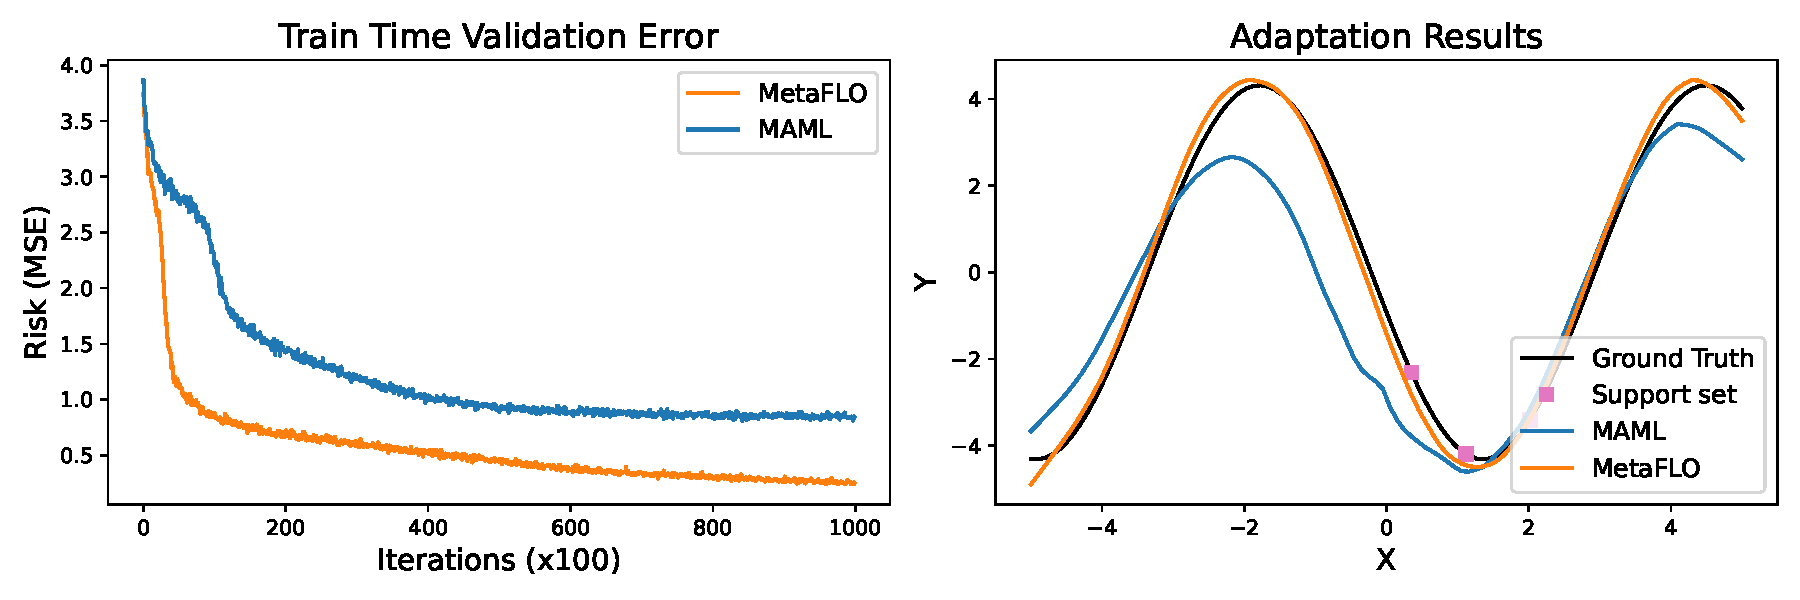
\includegraphics[width=.9\textwidth]{figures/toy/sin_no_noise}
}
\end{center}
\vskip -.1in
%\caption{.}
\caption{Meta regression with sine waves. (left) Train time validation MSE (right) Adaptation result with three supporting samples. \label{fig:sin_no_noise} We see MAML learns much slower than $\metaflo$, and the difference is more pronounced when viewed in runtime progress.}
\end{figure*}

\section{Experiments}

We consider different tasks to validate $\metaflo$ and benchmark it against state-of-the-art solutions. Details of experimental setups are described the Appendix. All experiments are implemented with PyTorch.
%, and our code is available from \url{https://github.com/author_name/MetaFLO}. 



\subsection{Regression}

We start with the synthetic regression problem from \citep{finn2017model} to illustrate the basic principles. Each task involves regressing from the input ($x\sim \text{Uniform}([-5,5])$) to the output of a sine wave $\kappa \sin(x-\gamma)$, where amplitude $\kappa \sim \text{Uniform}([0.1,5])$ and phase ($\gamma \sim \text{Uniform}([0,\pi]$) of the sinusoid vary for each task. We use mean-squared error (MSE) as our loss and set the support-size = $3$ and query-size = $2$. We use simple three-layer MLPs for all the models: regressor, prompt encoder, and $\FLO$ critics, with hidden units all set to $[512, 512]$. During training, we use an episode-size of $64$. For MAML, we use the first-order implementation (FOMAML), and set inner learning rate to $\alpha=10^{-4}$. For $\metaflo$, we set regularization strength to $\lambda=10^{-2}$. All meta-parameters are updated using Adam optimizer with a learning rate of $10^{-4}$ and we run training for $100k$ steps. We summarize the training dynamics and adaptation results in Figure \ref{fig:sin_no_noise}. In terms of the runtime, $\metaflo$ is about $10\times$ faster under our setup ($1,134$s V.S. $11,122$s). 

\subsection{$\metaflo$ as a nonparametric Bayesian learner}

We next demonstrate $\metaflo$'s capability to encode task uncertainties, a feature that is under-investigated in current literature. While calling for specialized efforts to onboard such capability \citep{yoon2018bayesian}, this comes naturally to $\metaflo$: for a fixed prompt input, the task code will be different each time you sample from the stochastic prompt encoding network, and using different task codes gives different realizations of model predictions. 
%We demonstrate this with the noisy sine wave model in Figure X. 

%We start with a simple regression problem that illustrates the basic principles of MAML. Each task involves regress- ing from the input to the output of a sine wave, where the amplitude and phase of the sinusoid are varied between tasks. Thus, p(T ) is continuous, where the amplitude varies within [0.1, 5.0] and the phase varies within [0, π], and the input and output both have a dimensionality of 1. During training and testing, datapoints x are sampled uni- formly from [−5.0, 5.0]. The loss is the mean-squared error between the prediction f(x) and true value. The regres- sor is a neural network model with 2 hidden layers of size 40 with ReLU nonlinearities. When training with MAML, we use one gradient update with K = 10 examples with a fixed step size α = 0.01, and use Adam as the meta- optimizer (Kingma & Ba, 2015). The baselines are like- wise trained with Adam. To evaluate performance, we fine- tune a single meta-learned model on varying numbers of K examples, and compare performance to two baselines: (a) pretraining on all of the tasks, which entails training a net- work to regress to random sinusoid functions and then, at test-time, fine-tuning with gradient descent on the K pro- vided points, using an automatically tuned step size, and (b) an oracle which receives the true amplitude and phase as input. In Appendix C, we show comparisons to addi- tional multi-task and adaptation methods.



\section{Conclusions}

We presented a novel meta/few-shot learning framework based on information-theoretic bounds. Our solution organically integrates variational contrastive learning to estimate the generalization error. 




\bibliography{metaflo}
\bibliographystyle{icml2022}


%%%%%%%%%%%%%%%%%%%%%%%%%%%%%%%%%%%%%%%%%%%%%%%%%%%%%%%%%%%%%%%%%%%%%%%%%%%%%%%
%%%%%%%%%%%%%%%%%%%%%%%%%%%%%%%%%%%%%%%%%%%%%%%%%%%%%%%%%%%%%%%%%%%%%%%%%%%%%%%
% APPENDIX
%%%%%%%%%%%%%%%%%%%%%%%%%%%%%%%%%%%%%%%%%%%%%%%%%%%%%%%%%%%%%%%%%%%%%%%%%%%%%%%
%%%%%%%%%%%%%%%%%%%%%%%%%%%%%%%%%%%%%%%%%%%%%%%%%%%%%%%%%%%%%%%%%%%%%%%%%%%%%%%
\newpage
\appendix
\onecolumn

\section*{Appendix}


{\bf MI estimation.} MI regularization is centre to Meta-FLO. While MI estimation has been extensively studied and there are many existing solutions, practical choices need to conform to a few constraints \& priorities listed below
\begin{itemize}
\item Must be sample-based: We only have data points of $\phi_t$ and $h_t$% non-parametric estimator
\item Differentiable: Learning signals must be back-propagated to the model
\item Robust to small batch learning: Only a handful of tasks can be loaded into memory
\item Low bias and variance
\end{itemize} 
With these constraints in mind, we choose to work with the recently proposed $\FLO$ mutual information estimator. $\FLO$ belongs to the family of nonparametric variational bounds of MI, where an auxiliary function $g_{\psi}$ known as the {\it variational critic} is introduced to derive a computationally tractable statistics that lower bounds MI. We summarize the FLO in Algorithm 1. 

%  \begin{algorithm}[H]
%%   \caption{Fenchel-InfoNCE}
%\caption{$\FLO$}
%   \label{alg:flo}
%\begin{algorithmic}
%%\small
%\STATE Empirical data $\hat{p}_d = \{ (x_i, y_i) \}_{i=1}^n$ \\
%[1pt]
%\STATE Model parameters $\Psi = (\theta, \phi)$ \\
%[1pt]
%\FOR{$t=1,2,\cdots$}
%\STATE Sample $i,i' \sim [n]$ \\
%[1pt]
%\STATE $u = u_{\phi}(x_i), g_{\oplus} = g_{\theta}(x_i, y_i)$, \\
%\STATE $g_{\ominus} = g_{\theta}(x_i, y_{i'})$\\
%[1pt]
%\STATE $\CF = u + \exp(-u+g_{\ominus}-g_{\oplus})$\\
%[1pt]
%$\Psi_{t} = \Psi_{t} - \eta_t \nabla_{\Psi} \CF$
%\ENDFOR\\
%\end{algorithmic}
%\end{algorithm}

Compared to other eligible candidates, $\FLO$ and its variants have been demonstrated to be more sample-efficient, thus delivering better empirical small-batch performance. On the theoretical side, $\FLO$ is tight and it is the only MI estimator that provably converges under mild technical conditions. $\FLO$ also takes a more generic formulation which allows it to subsume other popular MI estimators such as $\infonce$, $\NWJ$ and $\TUBA$ as special cases.  

A few important remarks are in order. First, it is known that only lower bounds are feasible for sample-based non-parametric MI estimation \footnote{For MI upper bounds, the exact likelihood will be needed for the joint and marginal distributions.}, so our objective $\CL_{\metaflo}$ is not strictly an upper bound to the expected generalization risk, but rather an approximation to it (because we are using the lower bounds for the MI term). Another potential pitfall is that while the mini-batch estimate of $\hat{I}_{\FLO}$ is unbiased, the term $\sqrt{\hat{I}_{\FLO}}$ appearing in the formal generalization bound is biased due to the square root transformation. \footnote{Additionally, since we are using low-dimensional embeddings for the task and dataset ($\Phi = F(W)$ and $H=G(S)$), we have $I(\Phi, H)\leq I(W,S)$ in virtue of the data processing inequality.}
%, which is infeasib
% 


{\bf RKHS embedding of support dataset.} Representation of probability distributions is an active research area in both probability theory and statistical machine learning. Alternative forms of the same distribution can have attractive properties for either theoretical analysis or computations. Seeking vectorization of empirical distributions, we apply the reproducing kernel Hilbert space (RKHS) embedding technique in this work. 

Let $\kappa(z, z')$ be a universal kernel, then the mapping $\mu^{\kappa} \triangleq \EE_{Z\sim \mu}[\kappa(\cdot, Z)]$ is injective. For simplicity hereafter, we suppress the dependence on kernel $\kappa$ in our notations. For each dataset $\hat{S}_t$, we have a functional $\hat{\mu}_t$ representing the empirical distribution $\hat{S}_t$. To map this (infinite-dimensional) functional to a finite-dimensional vector space, we evaluate $\hat{\mu}$ on a fixed set of reference points $\BZ^{\text{ref}} = \{ z_{j}^{\text{ref}} \}_{j=1}^r$. This gives us a mapping from empirical distributions to a vector space. Note that under this RKHS embedding scheme, the number of empirical samples for different tasks is allowed to vary. This adds more flexibility as in practical applications the task data is often imbalanced. 

\beq
\hat{\mu}_t = \frac{1}{K} \sum_{k=1}^K \kappa(\cdot, z_{t,k}), \quad {h}_t = [\hat{\mu}_t( z_{1}^{\text{ref}}), \cdots,  \hat{\mu}(z_{r}^{\text{ref}})]
\eeq


{\bf Detailed experiment setups.} Since the regression experiment has a fixed input size, instead of using the transformer architecture, we use fixed-size MLP. The model is trained on CPU-only servers. For image models, we use the GPU implementation and run it on Nvidia V100 GPUs. The simple MLP model yields a hold-out accuracy of $60\%$ for the omniglot benchmark. 




{\bf Embarrassingly simple meta-learning.} To allow the entire community to harvest the gains of $\metaflo$ with ease, we have implemented interfaces maximally automate the workflow, which renders $\metaflo$ embarrassingly simple for zero/few-shot applications. At its minimum, our $\metaflo$ API only requires the users to provide their own data-loader, feature encoder $\text{Enc}(x)$ ({\it e.g.}, \texttt{ResNet} for images and $\texttt{Transformer}$ or $\texttt{RNN}$ for texts), the output dimension $d_y$, the loss criterion $\ell(\hat{y}, y)$ ({\it e.g.}, \texttt{Cross-Entropy}, $\texttt{MSE}$), and the regularization strength $\lambda$. We provide an illustrative example in Algorithm \ref{alg:simple_flo}. 

\begin{algorithm}[t!]
%   \caption{Fenchel-InfoNCE}
\caption{Embarrassingly simple $\metaflo$}
   \label{alg:simple_flo}
\begin{algorithmic}
%\small
%\STATE Data $\{ S_i = \{ (x_{i,k}, y_{i,k}) \}_{k=1}^K \}_{i=1}^N$\\
%\STATE \texttt{class} WrapperMetaFLO()
\STATE \# User supplied components
\STATE x\_encoder = \texttt{ResNet}(image\_size), y\_dim = ...
\STATE data\_loader = CustomizedLoader(data) \# returns shape
\STATE \# [episode\_size, prompt/query\_size, data\_dims]
\STATE criterion = CrossEntropy(), $\lambda=0.01$
\STATE \# Enabling $\metaflo$
\STATE \# Optional args: optimizer, hidden dims, metrics, {\it etc.}
\STATE model = MetaFLO(x\_encoder, y\_dim, criterion, $\lambda$)
\FOR{$\text{step}=1,2,\cdots$}
\STATE \# Queries are paired data [x, y]
\STATE prompts, queries =  data\_loader.sample()
\STATE model.update(prompts, queries)
\ENDFOR
\STATE $\hat{y}$ = model.predict(prompts, x) \\
%[5pt]
%\STATE \# Advanced uses
%\STATE $\CL_R, \CL_{\FLO}$ = model(prompts, queries)
%\STATE $e$ = model.prompt\_encoder(prompts)
\end{algorithmic}
\end{algorithm}

%\section{You \emph{can} have an appendix here.}
%
%You can have as much text here as you want. The main body must be at most $8$ pages long.
%For the final version, one more page can be added.
%If you want, you can use an appendix like this one, even using the one-column format.
%%%%%%%%%%%%%%%%%%%%%%%%%%%%%%%%%%%%%%%%%%%%%%%%%%%%%%%%%%%%%%%%%%%%%%%%%%%%%%%
%%%%%%%%%%%%%%%%%%%%%%%%%%%%%%%%%%%%%%%%%%%%%%%%%%%%%%%%%%%%%%%%%%%%%%%%%%%%%%%


\end{document}


% This document was modified from the file originally made available by
% Pat Langley and Andrea Danyluk for ICML-2K. This version was created
% by Iain Murray in 2018, and modified by Alexandre Bouchard in
% 2019 and 2021 and by Csaba Szepesvari, Gang Niu and Sivan Sabato in 2022. 
% Previous contributors include Dan Roy, Lise Getoor and Tobias
% Scheffer, which was slightly modified from the 2010 version by
% Thorsten Joachims & Johannes Fuernkranz, slightly modified from the
% 2009 version by Kiri Wagstaff and Sam Roweis's 2008 version, which is
% slightly modified from Prasad Tadepalli's 2007 version which is a
% lightly changed version of the previous year's version by Andrew
% Moore, which was in turn edited from those of Kristian Kersting and
% Codrina Lauth. Alex Smola contributed to the algorithmic style files.
